% Options for packages loaded elsewhere
\PassOptionsToPackage{unicode}{hyperref}
\PassOptionsToPackage{hyphens}{url}
%
\documentclass[
  ignorenonframetext,
]{beamer}
\title{Explorative Faktorenanalyse}
\subtitle{Bißantz, Jalynskij, Kupffer \& Prestele}
\author{BF3 Testtheorie}
\date{}

\usepackage{pgfpages}
\setbeamertemplate{caption}[numbered]
\setbeamertemplate{caption label separator}{: }
\setbeamercolor{caption name}{fg=normal text.fg}
\beamertemplatenavigationsymbolsempty
% Prevent slide breaks in the middle of a paragraph
\widowpenalties 1 10000
\raggedbottom
\setbeamertemplate{part page}{
  \centering
  \begin{beamercolorbox}[sep=16pt,center]{part title}
    \usebeamerfont{part title}\insertpart\par
  \end{beamercolorbox}
}
\setbeamertemplate{section page}{
  \centering
  \begin{beamercolorbox}[sep=12pt,center]{part title}
    \usebeamerfont{section title}\insertsection\par
  \end{beamercolorbox}
}
\setbeamertemplate{subsection page}{
  \centering
  \begin{beamercolorbox}[sep=8pt,center]{part title}
    \usebeamerfont{subsection title}\insertsubsection\par
  \end{beamercolorbox}
}
\AtBeginPart{
  \frame{\partpage}
}
\AtBeginSection{
  \ifbibliography
  \else
    \frame{\sectionpage}
  \fi
}
\AtBeginSubsection{
  \frame{\subsectionpage}
}
\usepackage{amsmath,amssymb}
\usepackage{lmodern}
\usepackage{iftex}
\ifPDFTeX
  \usepackage[T1]{fontenc}
  \usepackage[utf8]{inputenc}
  \usepackage{textcomp} % provide euro and other symbols
\else % if luatex or xetex
  \usepackage{unicode-math}
  \defaultfontfeatures{Scale=MatchLowercase}
  \defaultfontfeatures[\rmfamily]{Ligatures=TeX,Scale=1}
\fi
\usetheme[]{Boadilla}
% Use upquote if available, for straight quotes in verbatim environments
\IfFileExists{upquote.sty}{\usepackage{upquote}}{}
\IfFileExists{microtype.sty}{% use microtype if available
  \usepackage[]{microtype}
  \UseMicrotypeSet[protrusion]{basicmath} % disable protrusion for tt fonts
}{}
\makeatletter
\@ifundefined{KOMAClassName}{% if non-KOMA class
  \IfFileExists{parskip.sty}{%
    \usepackage{parskip}
  }{% else
    \setlength{\parindent}{0pt}
    \setlength{\parskip}{6pt plus 2pt minus 1pt}}
}{% if KOMA class
  \KOMAoptions{parskip=half}}
\makeatother
\usepackage{xcolor}
\IfFileExists{xurl.sty}{\usepackage{xurl}}{} % add URL line breaks if available
\IfFileExists{bookmark.sty}{\usepackage{bookmark}}{\usepackage{hyperref}}
\hypersetup{
  pdftitle={Explorative Faktorenanalyse},
  pdfauthor={BF3 Testtheorie},
  hidelinks,
  pdfcreator={LaTeX via pandoc}}
\urlstyle{same} % disable monospaced font for URLs
\newif\ifbibliography
\usepackage{color}
\usepackage{fancyvrb}
\newcommand{\VerbBar}{|}
\newcommand{\VERB}{\Verb[commandchars=\\\{\}]}
\DefineVerbatimEnvironment{Highlighting}{Verbatim}{commandchars=\\\{\}}
% Add ',fontsize=\small' for more characters per line
\usepackage{framed}
\definecolor{shadecolor}{RGB}{248,248,248}
\newenvironment{Shaded}{\begin{snugshade}}{\end{snugshade}}
\newcommand{\AlertTok}[1]{\textcolor[rgb]{0.94,0.16,0.16}{#1}}
\newcommand{\AnnotationTok}[1]{\textcolor[rgb]{0.56,0.35,0.01}{\textbf{\textit{#1}}}}
\newcommand{\AttributeTok}[1]{\textcolor[rgb]{0.77,0.63,0.00}{#1}}
\newcommand{\BaseNTok}[1]{\textcolor[rgb]{0.00,0.00,0.81}{#1}}
\newcommand{\BuiltInTok}[1]{#1}
\newcommand{\CharTok}[1]{\textcolor[rgb]{0.31,0.60,0.02}{#1}}
\newcommand{\CommentTok}[1]{\textcolor[rgb]{0.56,0.35,0.01}{\textit{#1}}}
\newcommand{\CommentVarTok}[1]{\textcolor[rgb]{0.56,0.35,0.01}{\textbf{\textit{#1}}}}
\newcommand{\ConstantTok}[1]{\textcolor[rgb]{0.00,0.00,0.00}{#1}}
\newcommand{\ControlFlowTok}[1]{\textcolor[rgb]{0.13,0.29,0.53}{\textbf{#1}}}
\newcommand{\DataTypeTok}[1]{\textcolor[rgb]{0.13,0.29,0.53}{#1}}
\newcommand{\DecValTok}[1]{\textcolor[rgb]{0.00,0.00,0.81}{#1}}
\newcommand{\DocumentationTok}[1]{\textcolor[rgb]{0.56,0.35,0.01}{\textbf{\textit{#1}}}}
\newcommand{\ErrorTok}[1]{\textcolor[rgb]{0.64,0.00,0.00}{\textbf{#1}}}
\newcommand{\ExtensionTok}[1]{#1}
\newcommand{\FloatTok}[1]{\textcolor[rgb]{0.00,0.00,0.81}{#1}}
\newcommand{\FunctionTok}[1]{\textcolor[rgb]{0.00,0.00,0.00}{#1}}
\newcommand{\ImportTok}[1]{#1}
\newcommand{\InformationTok}[1]{\textcolor[rgb]{0.56,0.35,0.01}{\textbf{\textit{#1}}}}
\newcommand{\KeywordTok}[1]{\textcolor[rgb]{0.13,0.29,0.53}{\textbf{#1}}}
\newcommand{\NormalTok}[1]{#1}
\newcommand{\OperatorTok}[1]{\textcolor[rgb]{0.81,0.36,0.00}{\textbf{#1}}}
\newcommand{\OtherTok}[1]{\textcolor[rgb]{0.56,0.35,0.01}{#1}}
\newcommand{\PreprocessorTok}[1]{\textcolor[rgb]{0.56,0.35,0.01}{\textit{#1}}}
\newcommand{\RegionMarkerTok}[1]{#1}
\newcommand{\SpecialCharTok}[1]{\textcolor[rgb]{0.00,0.00,0.00}{#1}}
\newcommand{\SpecialStringTok}[1]{\textcolor[rgb]{0.31,0.60,0.02}{#1}}
\newcommand{\StringTok}[1]{\textcolor[rgb]{0.31,0.60,0.02}{#1}}
\newcommand{\VariableTok}[1]{\textcolor[rgb]{0.00,0.00,0.00}{#1}}
\newcommand{\VerbatimStringTok}[1]{\textcolor[rgb]{0.31,0.60,0.02}{#1}}
\newcommand{\WarningTok}[1]{\textcolor[rgb]{0.56,0.35,0.01}{\textbf{\textit{#1}}}}
\usepackage{graphicx}
\makeatletter
\def\maxwidth{\ifdim\Gin@nat@width>\linewidth\linewidth\else\Gin@nat@width\fi}
\def\maxheight{\ifdim\Gin@nat@height>\textheight\textheight\else\Gin@nat@height\fi}
\makeatother
% Scale images if necessary, so that they will not overflow the page
% margins by default, and it is still possible to overwrite the defaults
% using explicit options in \includegraphics[width, height, ...]{}
\setkeys{Gin}{width=\maxwidth,height=\maxheight,keepaspectratio}
% Set default figure placement to htbp
\makeatletter
\def\fps@figure{htbp}
\makeatother
\setlength{\emergencystretch}{3em} % prevent overfull lines
\providecommand{\tightlist}{%
  \setlength{\itemsep}{0pt}\setlength{\parskip}{0pt}}
\setcounter{secnumdepth}{-\maxdimen} % remove section numbering
\newlength{\cslhangindent}
\setlength{\cslhangindent}{1.5em}
\newlength{\csllabelwidth}
\setlength{\csllabelwidth}{3em}
\newlength{\cslentryspacingunit} % times entry-spacing
\setlength{\cslentryspacingunit}{\parskip}
\newenvironment{CSLReferences}[2] % #1 hanging-ident, #2 entry spacing
 {% don't indent paragraphs
  \setlength{\parindent}{0pt}
  % turn on hanging indent if param 1 is 1
  \ifodd #1
  \let\oldpar\par
  \def\par{\hangindent=\cslhangindent\oldpar}
  \fi
  % set entry spacing
  \setlength{\parskip}{#2\cslentryspacingunit}
 }%
 {}
\usepackage{calc}
\newcommand{\CSLBlock}[1]{#1\hfill\break}
\newcommand{\CSLLeftMargin}[1]{\parbox[t]{\csllabelwidth}{#1}}
\newcommand{\CSLRightInline}[1]{\parbox[t]{\linewidth - \csllabelwidth}{#1}\break}
\newcommand{\CSLIndent}[1]{\hspace{\cslhangindent}#1}
\ifLuaTeX
  \usepackage{selnolig}  % disable illegal ligatures
\fi

\begin{document}
\frame{\titlepage}

\begin{frame}[allowframebreaks]
  \tableofcontents[hideallsubsections]
\end{frame}
\hypertarget{einstieg}{%
\section*{Einstieg}\label{einstieg}}
\addcontentsline{toc}{section}{Einstieg}

\begin{frame}{Einstieg}
\begin{example}
Hinter unterstehendem Link verbirgt sich ein Fragebogen der Platform
\texttt{openpsychometrics} (eine gute Quelle um kostenlos Datensätze für
Analysen zu ergattern). Schauen Sie sich den Big-Five-Fragebogen einmal an. Wenn
Sie möchten, beantworten Sie Ihn kurz. Im Anschluss daran stellen wir uns auf
dieser Grundlage der Large Dataset Challenge!
\end{example}

\url{https://openpsychometrics.org/tests/IPIP-BFFM/}\footnote<.->{Für
  das Projekt, siehe: \url{https://openpsychometrics.org/}}

\begin{itemize}
\tightlist
\item
  Zeit: 2-3 Minuten
\end{itemize}
\end{frame}

\hypertarget{die-large-data-set-challenge}{%
\section{Die ``Large Data Set
Challenge''}\label{die-large-data-set-challenge}}

\begin{frame}{Die ``Large Data Set Challenge''}
\begin{example}
Stellen Sie sich vor, die von Ihnen soeben gesehenen/beantworteten Fragen
ergäben die Korrelationsmatrix $R$ auf der nächsten Folie. Die "Large Data Set
Challenge" (LDC) lautet: Erkennen Sie eine Struktur in den Daten? Das heißt
konkreter, finden Sie homogene Itemgruppen? Besprechen Sie sich mit ihrem
Nachbarn.
\end{example}

Welche Items könnte man ihrer Meinung nach zu Itemgruppen
zusammenfassen?

\begin{itemize}
\tightlist
\item
  Zeit: 2-3 Minuten
\end{itemize}

Anmerkung: Nein, das sind nicht ihre Antworten; \(\texttt{V1 - V25}\)
sind Zufallsvariablen!
\end{frame}

\begin{frame}{Übungsaufgabe 1: Struktur erkennen \& Itemgruppen finden}
\protect\hypertarget{uxfcbungsaufgabe-1-struktur-erkennen-itemgruppen-finden}{}
\begin{center}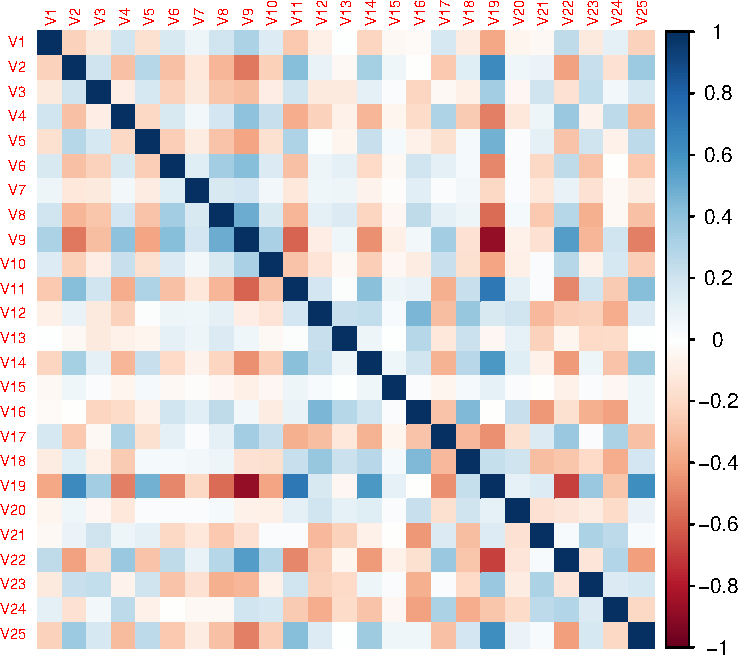
\includegraphics[width=0.7\linewidth]{06-EFA_files/figure-beamer/unnamed-chunk-1-1} \end{center}
\end{frame}

\begin{frame}{Die ``Large Data Set Challenge'' (..in theory)}
\protect\hypertarget{die-large-data-set-challenge-..in-theory}{}
\begin{alertblock}{Large Data Set Challenge}
Mit zunehmender Itemzahl nimmt die Anzahl der Korrelationen, die für eine
Analyse zu berücksichtigen sind schnell zu groß. Die "Challenge" ist eine
mögliche Struktur zu entdecken! (..Wie sie eben in ihrer visuellen Zuordnungen
selbst gemerkt haben)
\end{alertblock}

In a Nutshell:

\begin{itemize}
\tightlist
\item
  Problem: Anzahl der Korrelationen
\item
  z.B.: \(25\) Items \(\widehat{=}\) 300 Korrelationen
\item
  Krux: Struktur erkennen
\item
  \(\Leftrightarrow\) finde: hoch korrelierende Itemgruppen
\end{itemize}
\end{frame}

\begin{frame}{Explorative Faktorenanalyse \& Large Data Set Challenge}
\protect\hypertarget{explorative-faktorenanalyse-large-data-set-challenge}{}
\begin{itemize}
\tightlist
\item
  (ein) Hilfsmittel für die LDC: (explorative) \emph{Faktorenanalyse}
\end{itemize}

\begin{itemize}
\item
  andere Helferlein zur \emph{Datenreduktion} (eine Auswahl):

  \begin{itemize}
  \tightlist
  \item
    Hauptkomponentenanalyse
  \item
    Clusteranalyse
  \item
    Explorative Likertskalierung
  \item
    (Non-) Metric Data Scaling (Distanzmatrizen!)
  \end{itemize}
\end{itemize}

Wichtig: ``meaningful'' (Faktoren) vs.~``full compression''
(Komponenten)

Fokus (heute): Hauptkomponentenanalyse (PCA), Hauptachsenanalyse (PAF),
Maximum Likelihood Faktorenanalyse (MLF)
\end{frame}

\hypertarget{fakotrenanalyse-a-hurdle-race}{%
\section{Fakotrenanalyse: ``A hurdle
race''}\label{fakotrenanalyse-a-hurdle-race}}

\begin{frame}{Fakotrenanalyse: ``A hurdle race''}
\begin{enumerate}
\tightlist
\item
  Hürde: Extraktionsproblem
\item
  Hürde: Rotationsproblem
\item
  Hürde: Problem der Anzahl zu extrahierender Faktoren
\end{enumerate}

~

\begin{quote}
``Unfortunately, factor analysis is frequently misunderstood and often
misused. Some researchers appear to use factor analysis as a kind of
divining rod, hoping to find gold hidden underneath tons of dirt. But
there is nothing magical about the technique. {[}\(\dots\){]} Factor
analysis will yield meaningful results only when the research was
meaningful to begin with.''
\href{https://www.pearson.com/us/higher-education/program/Gregory-Psychological-Testing-History-Principles-and-Applications-7th-Edition/PGM332874.html}{Gregory
(2014, S. 165)}
\end{quote}

Konkl.: Versuchen Sie ihr Modell zu verstehen! (siehe: Selbststudium)
\end{frame}

\begin{frame}[fragile]{Vorbereitung: ``Playing Creator'' -- 2 LVs
erschaffen}
\protect\hypertarget{vorbereitung-playing-creator-2-lvs-erschaffen}{}
Bevor wir loslegen, wollen wir eine Datenmatrix \(X\) und eine
Korrelationsmatrix \(R\) simulieren.\footnote<.->{Nur in simulierten
  Welten (in denen wir den richtigen Ausgang kennen), können wir prüfen,
  ob unsere Methoden das ``korrekte'' Ergebnis reproduzieren. Sie können
  sich aber auch vorstellen, dass das Ihre Antworten auf den Fragebogen
  seien. Dann wären Sie der generative Prozess, den wir hier simulieren.}

\begin{Shaded}
\begin{Highlighting}[]
\CommentTok{\# Faktorladungen; 8 items}
\NormalTok{load\_F1 }\OtherTok{\textless{}{-}} \FunctionTok{c}\NormalTok{(}\FloatTok{0.6}\NormalTok{, }\SpecialCharTok{{-}}\FloatTok{0.3}\NormalTok{, }\FloatTok{0.5}\NormalTok{, }\FloatTok{0.7}\NormalTok{, }\FloatTok{0.1}\NormalTok{, }\FloatTok{0.2}\NormalTok{, }\FloatTok{0.2}\NormalTok{, }\FloatTok{0.3}\NormalTok{)}
\NormalTok{load\_F2 }\OtherTok{\textless{}{-}} \FunctionTok{c}\NormalTok{(}\SpecialCharTok{{-}}\FloatTok{0.1}\NormalTok{, }\FloatTok{0.1}\NormalTok{, }\FloatTok{0.1}\NormalTok{, }\FloatTok{0.1}\NormalTok{, }\SpecialCharTok{{-}}\FloatTok{0.7}\NormalTok{, }\FloatTok{0.5}\NormalTok{, }\SpecialCharTok{{-}}\FloatTok{0.6}\NormalTok{, }\FloatTok{0.7}\NormalTok{)}
\NormalTok{fx }\OtherTok{\textless{}{-}} \FunctionTok{cbind}\NormalTok{(load\_F1, load\_F2)}
\CommentTok{\# Zwischenfaktorkorrelation }
\NormalTok{phi }\OtherTok{\textless{}{-}} \FunctionTok{diag}\NormalTok{(}\FunctionTok{rep}\NormalTok{(}\DecValTok{1}\NormalTok{, }\DecValTok{2}\NormalTok{)) ; phi[}\DecValTok{1}\NormalTok{, }\DecValTok{2}\NormalTok{] }\OtherTok{\textless{}{-}}\NormalTok{ phi[}\DecValTok{2}\NormalTok{, }\DecValTok{1}\NormalTok{] }\OtherTok{\textless{}{-}} \FloatTok{0.6}
\CommentTok{\# Struktur }
\NormalTok{S }\OtherTok{\textless{}{-}}\NormalTok{ psych}\SpecialCharTok{::}\FunctionTok{sim.structure}\NormalTok{(fx, phi, }\AttributeTok{n=}\DecValTok{1000}\NormalTok{)}
\CommentTok{\# Korrelations{-} und Datenmatrix}
\NormalTok{R }\OtherTok{\textless{}{-}}\NormalTok{ S}\SpecialCharTok{$}\NormalTok{model ; X }\OtherTok{\textless{}{-}}\NormalTok{ S}\SpecialCharTok{$}\NormalTok{observed  }\CommentTok{\# R \textless{}{-} cor(X)}
\end{Highlighting}
\end{Shaded}
\end{frame}

\hypertarget{extraktionsproblem}{%
\section{Extraktionsproblem}\label{extraktionsproblem}}

\begin{frame}{Extraktionsproblem}
\begin{alertblock}{Extraktionsproblem}
  Wie extrahieren wir die zur Reproduktion nötigen Faktoren/Komponenten?
\end{alertblock}

\begin{enumerate}
\tightlist
\item
  Lösung: Bestimmung der ``Principal Components''
  (\emph{PCA})\footnote<.->{Faktoren- und Hauptkomponentenanylse sind
    Verfahren mit unterschiedlichen Zielen! Beide Klassen nutzen
    unterschiedliche Modelle und machen unterschiedliche Basisannahmen.
    Dennoch werden sie häufig in der Literatur unter dem Deckmantel
    ``explorative Faktorenanalyse'' vereinheitlicht.}
\item
  Lösung: Iterative Bestimmung der ``Principal Components'' (\emph{PAF})
\item
  Lösung: Finde die plausibelsten (``most likely'') Werte (\emph{MLF})
\end{enumerate}
\end{frame}

\begin{frame}[fragile]{Let's do it! (..in R): PCA}
\protect\hypertarget{lets-do-it-..in-r-pca}{}
\begin{Shaded}
\begin{Highlighting}[]
\CommentTok{\# Old School!}
\CommentTok{\# (dino\_pca \textless{}{-} princomp(X, cor=TRUE))}
\CommentTok{\# New School: Datenmatrix? R {-}\textgreater{} X}
\NormalTok{(fit\_pca }\OtherTok{\textless{}{-}}\NormalTok{ psych}\SpecialCharTok{::}\FunctionTok{principal}\NormalTok{(R, }\AttributeTok{nfactors =} \DecValTok{2}\NormalTok{, }
                            \AttributeTok{rotate =} \StringTok{"none"}\NormalTok{))}

\DocumentationTok{\#\# Komponentenladungen}
\NormalTok{fit\_pca}\SpecialCharTok{$}\NormalTok{loadings}
\DocumentationTok{\#\# Kommunalitäten }
\NormalTok{fit\_pca}\SpecialCharTok{$}\NormalTok{communality}
\DocumentationTok{\#\# Einzigartigkeit }
\NormalTok{fit\_pca}\SpecialCharTok{$}\NormalTok{uniquenesses}
\DocumentationTok{\#\# Eigenwerte}
\NormalTok{fit\_pca}\SpecialCharTok{$}\NormalTok{values}
\CommentTok{\# Quadrierte multiple Korrelation}
\NormalTok{fit\_pca}\SpecialCharTok{$}\NormalTok{R2}
\end{Highlighting}
\end{Shaded}
\end{frame}

\begin{frame}{Übungsaufgabe 2: Selbstexperiment}
\protect\hypertarget{uxfcbungsaufgabe-2-selbstexperiment}{}
\begin{example}
Versuchen Sie es nun selbst! Nutzen Sie den Code zur Übungsaufgabe 2
\texttt{06-EFA.R} und führen eine PCA durch. Interpretieren Sie die
entsprechenden Kennwerte für ihr Modell und präsentieren Sie diese ihrem
Nachbarn.
\end{example}

\begin{itemize}
\tightlist
\item
  Zeit: 10 Minuten
\item
  Replikation: \texttt{set.seed(123)}
\item
  Anmerkung: Konzepte \& Output verstehen \(\gg\) Codes verstehen!
\end{itemize}

Anmerkung: Normalerweise kennen Sie die Anzahl der zu extrahierenden
Komponenten/Faktoren nicht. Wie man dieses Problem angeht, dazu gleich
mehr!
\end{frame}

\begin{frame}[fragile]{Let's do it! (..in R): Hauptachsenanalyse (PAF)}
\protect\hypertarget{lets-do-it-..in-r-hauptachsenanalyse-paf}{}
\begin{Shaded}
\begin{Highlighting}[]
\NormalTok{(fit\_paf }\OtherTok{\textless{}{-}}\NormalTok{ psych}\SpecialCharTok{::}\FunctionTok{fa}\NormalTok{(R, }\AttributeTok{nfactors=}\DecValTok{2}\NormalTok{,}
                      \AttributeTok{rotate=}\StringTok{"none"}\NormalTok{,}
                      \AttributeTok{fm=}\StringTok{"pa"}\NormalTok{))}
\CommentTok{\# Kommunalitäten}
\NormalTok{fit\_paf}\SpecialCharTok{$}\NormalTok{communality}
\CommentTok{\# Eigenwerte}
\NormalTok{fit\_paf}\SpecialCharTok{$}\NormalTok{e.values}
\CommentTok{\# Einzigartigkeit}
\NormalTok{fit\_paf}\SpecialCharTok{$}\NormalTok{uniquenesses}
\CommentTok{\# Quadrierte multiple Korrelation}
\NormalTok{fit\_paf}\SpecialCharTok{$}\NormalTok{R2}
\end{Highlighting}
\end{Shaded}
\end{frame}

\begin{frame}{Übungsaufgabe 3: Selbstexperiment}
\protect\hypertarget{uxfcbungsaufgabe-3-selbstexperiment}{}
\begin{example}
Versuchen Sie es nun selbst! Nutzen Sie den Code zur Übungsaufgabe 3
\texttt{06-EFA.R} und führen Sie eine Hauptachsenanalyse (PAF) durch.
Vergleichen Sie die Ergebnisse der PAF mit denen der PCA. Bestehen Unterschiede
zwischen den Ergebnissen? 
\end{example}

\begin{itemize}
\tightlist
\item
  Zeit: 10 Minuten
\item
  Replikation: \texttt{set.seed(123)}
\item
  Anmerkung: Konzepte \& Output verstehen \(\gg\) Codes verstehen!
\end{itemize}
\end{frame}

\begin{frame}{Primer: Maximum Likelihood Faktorenanalyse (MLF)}
\protect\hypertarget{primer-maximum-likelihood-faktorenanalyse-mlf}{}
MLF bietet als Lösung die plausibelsten (eng. ``most likely'')
(Parameter-) Werte zur Reproduktion der Informationen in der
Korrelationsmatrix an.

\begin{equation}
  X_i = \lambda_j*\xi_i + \epsilon_i
\end{equation}

\begin{equation}
  R^* = \Lambda \Phi \Lambda' + \Psi
\end{equation}

\begin{itemize}
\tightlist
\item
  \(R\): Korrelationsmatrix
\item
  \(X_i\): Item \(i\)
\item
  \(\lambda, \Lambda\): Ladung, Ladungsmatrix
\item
  \(\xi\): Faktor
\item
  \(\Phi\): Zwischenfaktorkorrelationsmatrix
\item
  \(\Psi\): Einzigartigkeit
\end{itemize}
\end{frame}

\begin{frame}[fragile]{Let's do it (..in R): Maximum Likelihood
Faktorenanalyse (MLF)}
\protect\hypertarget{lets-do-it-..in-r-maximum-likelihood-faktorenanalyse-mlf}{}
\begin{Shaded}
\begin{Highlighting}[]
\NormalTok{(fit\_mlf }\OtherTok{\textless{}{-}}\NormalTok{ psych}\SpecialCharTok{::}\FunctionTok{fa}\NormalTok{(R, }\AttributeTok{nfactors=}\DecValTok{2}\NormalTok{,}
                      \AttributeTok{rotate=}\StringTok{"none"}\NormalTok{,}
                      \AttributeTok{fm=}\StringTok{"ml"}\NormalTok{))}
\CommentTok{\# Kommunalitäten}
\NormalTok{fit\_mlf}\SpecialCharTok{$}\NormalTok{communality}
\CommentTok{\# Eigenwerte}
\NormalTok{fit\_mlf}\SpecialCharTok{$}\NormalTok{e.values}
\CommentTok{\# Einzigartigkeit}
\NormalTok{fit\_mlf}\SpecialCharTok{$}\NormalTok{uniquenesses}
\CommentTok{\# Quadrierte multiple Korrelation}
\NormalTok{fit\_mlf}\SpecialCharTok{$}\NormalTok{R2}
\end{Highlighting}
\end{Shaded}
\end{frame}

\begin{frame}{Übungsaufgabe 4: Selbstexperiment}
\protect\hypertarget{uxfcbungsaufgabe-4-selbstexperiment}{}
\begin{example}
Versuchen Sie es nun selbst! Nutzen Sie den Code zur Übungsaufgabe 4 in
\texttt{06-EFA.R} und führen Sie eine Maximum Likelihood Faktorenanalyse (MLF)
durch. Vergleichen Sie die Ergebnisse auch mit den anderen Methoden.
\end{example}

\begin{itemize}
\tightlist
\item
  Zeit: 10 Minuten
\item
  Replikation: \texttt{set.seed(123)}
\item
  Anmerkung: Konzepte \& Output verstehen \(\gg\) Codes verstehen!
\end{itemize}
\end{frame}

\hypertarget{rotationsproblem}{%
\section{Rotationsproblem}\label{rotationsproblem}}

\begin{frame}{Rotationsproblem}
\begin{alertblock}{Rotationsproblem}
  Wie rotiert die erhaltene Ladungsmatrix ($\hat\Lambda$) derart, dass eine
  möglich einfach interpretierbare Lösung daraus hervorgeht?
\end{alertblock}

\begin{enumerate}
\tightlist
\item
  Lösung: orthogonale Rotation
\item
  Lösung: oblique Rotation
\end{enumerate}
\end{frame}

\begin{frame}{Graphik: Orthogonale Rotation mit Varimax}
\protect\hypertarget{graphik-orthogonale-rotation-mit-varimax}{}
\includegraphics{06-EFA_files/figure-beamer/unnamed-chunk-6-1.pdf}
\end{frame}

\begin{frame}{Graphik: Oblique Rotation mit Oblimin}
\protect\hypertarget{graphik-oblique-rotation-mit-oblimin}{}
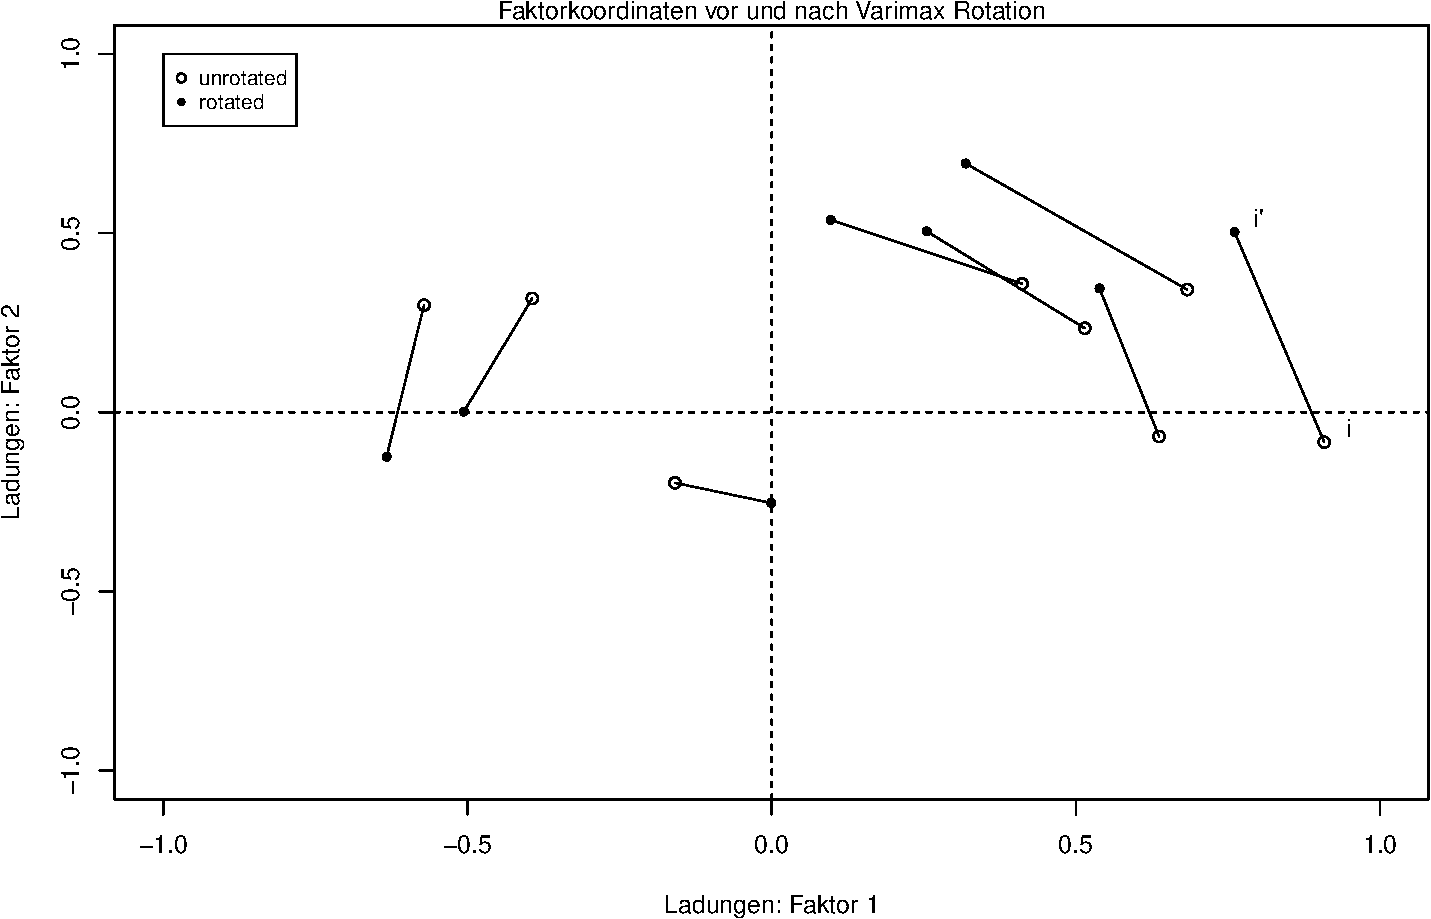
\includegraphics{06-EFA_files/figure-beamer/unnamed-chunk-7-1.pdf}
\end{frame}

\begin{frame}[fragile]{Let's do it (..in R): orthogonale Rotation
(Varimax)}
\protect\hypertarget{lets-do-it-..in-r-orthogonale-rotation-varimax}{}
\begin{Shaded}
\begin{Highlighting}[]
\NormalTok{(fit\_vmax }\OtherTok{\textless{}{-}}\NormalTok{ psych}\SpecialCharTok{::}\FunctionTok{fa}\NormalTok{(R, }\AttributeTok{nfactors=}\DecValTok{2}\NormalTok{,}
                       \AttributeTok{rotate=}\StringTok{"varimax"}\NormalTok{,}
                       \AttributeTok{fm=}\StringTok{"ml"}\NormalTok{))}
\CommentTok{\# Kommunalitäten}
\NormalTok{fit\_vmax}\SpecialCharTok{$}\NormalTok{communality}
\CommentTok{\# Eigenwerte}
\NormalTok{fit\_vmax}\SpecialCharTok{$}\NormalTok{e.values}
\CommentTok{\# Einzigartigkeit}
\NormalTok{fit\_vmax}\SpecialCharTok{$}\NormalTok{uniquenesses}
\CommentTok{\# Quadrierte multiple Korrelation}
\NormalTok{fit\_vmax}\SpecialCharTok{$}\NormalTok{R2}
\end{Highlighting}
\end{Shaded}
\end{frame}

\begin{frame}[fragile]{Let's do it (..in R): oblique Rotation (Oblimin)}
\protect\hypertarget{lets-do-it-..in-r-oblique-rotation-oblimin}{}
\begin{Shaded}
\begin{Highlighting}[]
\NormalTok{(fit\_obl }\OtherTok{\textless{}{-}}\NormalTok{ psych}\SpecialCharTok{::}\FunctionTok{fa}\NormalTok{(R, }\AttributeTok{nfactors=}\DecValTok{2}\NormalTok{,}
                      \AttributeTok{rotate=}\StringTok{"oblimin"}\NormalTok{,}
                      \AttributeTok{fm=}\StringTok{"ml"}\NormalTok{))}
\CommentTok{\# Kommunalitäten}
\NormalTok{fit\_obl}\SpecialCharTok{$}\NormalTok{communality}
\CommentTok{\# Eigenwerte}
\NormalTok{fit\_obl}\SpecialCharTok{$}\NormalTok{e.values}
\CommentTok{\# Einzigartigkeit}
\NormalTok{fit\_obl}\SpecialCharTok{$}\NormalTok{uniquenesses}
\CommentTok{\# Quadrierte multiple Korrelation}
\NormalTok{fit\_obl}\SpecialCharTok{$}\NormalTok{R2}
\CommentTok{\# Wichtig: Phi}
\NormalTok{fit\_obl}\SpecialCharTok{$}\NormalTok{Phi}
\end{Highlighting}
\end{Shaded}
\end{frame}

\begin{frame}{Übungsaufgabe 5: Selbstexperiment}
\protect\hypertarget{uxfcbungsaufgabe-5-selbstexperiment}{}
\begin{example}
Versuchen Sie es nun selbst! Nutzen Sie den Code zur Übungsaufgabe 5 in
\texttt{06-EFA.R} und führen Sie eine MLF durch. Rotieren Sie anschließend die
Ergebnisse mit der Varimax und Oblimin Rotation. Wie verändert die Rotation ihre
Interpretation der Ergebnisse? Erleichtert sie sie? Vergleichen Sie die Lösung
dazu (1) mit der unrotierten Lösung und vergleichen Sie (2) die Ergebnisse
zwischend den Rotationsmethoden.
\end{example}

\begin{itemize}
\tightlist
\item
  Zeit: 10 Minuten
\item
  Replikation: \texttt{set.seed(123)}
\item
  Anmerkung: Konzepte \& Output verstehen \(\gg\) Codes verstehen!
\end{itemize}
\end{frame}

\begin{frame}{Übungsaufgabe 6: Kritische Reflexion \& Diskussion}
\protect\hypertarget{uxfcbungsaufgabe-6-kritische-reflexion-diskussion}{}
\begin{example}
Eine Folge der orthogonalen Rotation ist, dass die extrahierten Faktoren
unabhängig voneinander sind. Glauben Sie dem Modell uneingeschränkt, nähmen sie
damit implizit an, dass auch die zugrundeliegende Konstrukte unabhängig
voneinander sein müssten. Für wie plausibel halten Sie diese Annahme in der
Psychologie? Diskutieren Sie miteinander!
\end{example}

\begin{itemize}
\tightlist
\item
  Zeit: 2-3 Minuten
\end{itemize}
\end{frame}

\hypertarget{problem-der-anzahl-zu-extrahierender-faktoren}{%
\section{Problem der Anzahl zu extrahierender
Faktoren}\label{problem-der-anzahl-zu-extrahierender-faktoren}}

\begin{frame}{Problem der Anzahl zu extrahierender Faktoren}
\begin{alertblock}{Rotationsproblem}
  Wie ermittle ich die Anzahl der zu extrahierenden Faktoren ohne sie zu kennen?
\end{alertblock}

\begin{enumerate}
\tightlist
\item
  Lösung: Kaiser Kriterium
\item
  Lösung: Scree-Test
\item
  Lösung. Horns Parallel Analyse\footnote<.->{Es gibt mittlerweile
    zahlreiche Weiterentwicklungen. Interessieren Sie sich dafür? Dann
    schauen Sie in
    \href{https://sci-hub.se/10.1080/00273171.2011.564527}{Lorenzo-Seva
    et al.~(2011)} \&
    \href{https://doi.org/10.1002/9781118489772.ch11}{Timmerman et
    al.~(2018)}.}
\end{enumerate}
\end{frame}

\begin{frame}{Eigenwerteplots (Kaiser Kriterium \& Scree Test)}
\protect\hypertarget{eigenwerteplots-kaiser-kriterium-scree-test}{}
\begin{block}{Kaiserkriterium \& Scree Test}
Zerlege die Korrelationsmatrix in ihre Eigenwerte (SVD/EVD) und plotte diese
gegen einen Index.
\begin{enumerate}
  \item Kaiserkriterium: Ist das Varianzaufklärungspotential eines Faktors kleiner als das eines Items beende deine Suche ($\widetilde{=}EW > 1$). 
  \item Scree-Test: Finde den "ellbow" der den "rock" vom "scree" unterscheidet.
\end{enumerate}
\end{block}
\end{frame}

\begin{frame}{Grafik: Eigenwertplot}
\protect\hypertarget{grafik-eigenwertplot}{}
\includegraphics{06-EFA_files/figure-beamer/unnamed-chunk-10-1.pdf}
\end{frame}

\begin{frame}[fragile]{Let's do it (..in R): Eigenwerteplots}
\protect\hypertarget{lets-do-it-..in-r-eigenwerteplots}{}
\begin{Shaded}
\begin{Highlighting}[]
\CommentTok{\# Barfuß}
\NormalTok{ ev }\OtherTok{\textless{}{-}} \FunctionTok{eigen}\NormalTok{(R)}\SpecialCharTok{$}\NormalTok{values}
 \FunctionTok{plot}\NormalTok{(ev, }\AttributeTok{main=}\StringTok{"Eigenwerteplot"}\NormalTok{, }\AttributeTok{xlab=}\StringTok{"Eigenwerte"}\NormalTok{,}
      \AttributeTok{ylab =} \StringTok{"Komponentenzahl"}\NormalTok{, }\AttributeTok{type=}\StringTok{"b"}\NormalTok{)}
 \FunctionTok{abline}\NormalTok{(}\AttributeTok{h=}\DecValTok{1}\NormalTok{, }\AttributeTok{lty=}\DecValTok{2}\NormalTok{)}

\CommentTok{\# psych package}
\NormalTok{psych}\SpecialCharTok{::}\FunctionTok{scree}\NormalTok{(R, }\AttributeTok{factors =} \ConstantTok{FALSE}\NormalTok{)}
\CommentTok{\# psych::scree(R, factors = TRUE)}
\end{Highlighting}
\end{Shaded}
\end{frame}

\begin{frame}{Parallel Analyse}
\protect\hypertarget{parallel-analyse}{}
\begin{alertblock}{Parallel Analyse}
"In parallel analysis, the criterion to be used in order to determine the number
of factors is the following A factor is considered as "significant" if its
eigenvalue is larger than the 95\% quantile [...] of those obtained from
random or resampled data." (Mair 2018, S.31)
\end{alertblock}

Anmerkung: Im Orginal wurde die PA für Komponenten konstruiert.
Mittlerweile gibt es sie auch für das CFM.
\end{frame}

\begin{frame}[fragile]{Grafik: Parallel Analyse (PCA)}
\protect\hypertarget{grafik-parallel-analyse-pca}{}
\begin{verbatim}
## 
## Using eigendecomposition of correlation matrix.
\end{verbatim}

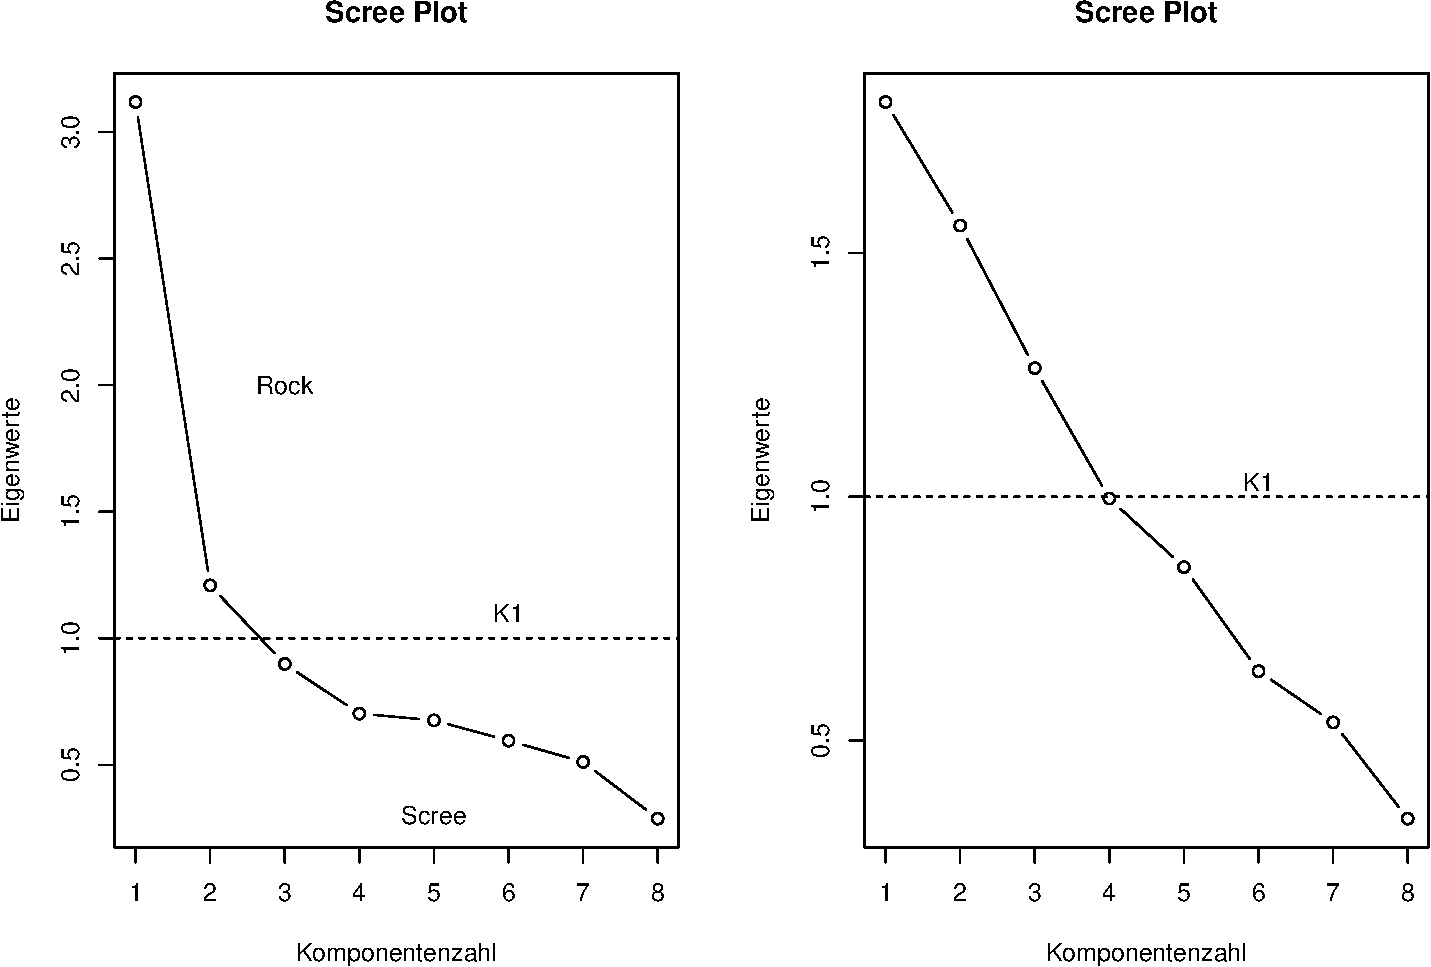
\includegraphics[width=0.7\linewidth]{06-EFA_files/figure-beamer/unnamed-chunk-12-1}

Anmerkung: Die Grafik wurde mit \(\texttt{paran}\) nicht
\(\texttt{psych}\) erstellt.
\end{frame}

\begin{frame}[fragile]{Grafik: Parallel Analyse (FA)}
\protect\hypertarget{grafik-parallel-analyse-fa}{}
\begin{verbatim}
## 
## Using eigendecomposition of correlation matrix.
\end{verbatim}

\includegraphics[width=0.7\linewidth]{06-EFA_files/figure-beamer/unnamed-chunk-13-1}

Anmerkung: Die Grafik wurde mit \(\texttt{paran}\) nicht
\(\texttt{psych}\) erstellt.
\end{frame}

\begin{frame}[fragile]{Let's do it (..in R): Parallel Analyse}
\protect\hypertarget{lets-do-it-..in-r-parallel-analyse}{}
\begin{Shaded}
\begin{Highlighting}[]
\CommentTok{\# Parallelanalyse (Komponenten{-}basiert)}
\NormalTok{psych}\SpecialCharTok{::}\FunctionTok{fa.parallel}\NormalTok{(X, }\AttributeTok{fa =} \StringTok{"pc"}\NormalTok{, }\AttributeTok{fm =} \StringTok{"ml"}\NormalTok{)}

\CommentTok{\# Alternative}
\CommentTok{\#}
\CommentTok{\# Für Komponenten}
\CommentTok{\# paran::paran(X)}
\CommentTok{\# Für Faktoren}
\CommentTok{\# paran::paran(X, cfa=TRUE)}
\end{Highlighting}
\end{Shaded}
\end{frame}

\begin{frame}{Übungsaufgabe 7: Selbstexperiment}
\protect\hypertarget{uxfcbungsaufgabe-7-selbstexperiment}{}
\begin{example}
Versuchen Sie es nun selbst! Nutzen Sie den Code zur Übungsaufgabe 7 in
\texttt{06-EFA.R} und finden Sie die Anzahl zu extrahierender Faktoren in ihrem
Beispiel mit den drei genannten Möglichkeiten. Welches der drei Verfahren
"errät" die Anzahl zu extrahierender Faktoren aus der Simulation (2 Faktoren)? 
\end{example}

\begin{itemize}
\tightlist
\item
  Zeit: 10 Minuten
\item
  Replikation: \texttt{set.seed(123)}
\item
  Anmerkung: Konzepte \& Output verstehen \(\gg\) Codes verstehen!
\end{itemize}
\end{frame}

\hypertarget{bonusmaterial-bartlett-test-kmo}{%
\section{Bonusmaterial: Bartlett-Test \&
KMO}\label{bonusmaterial-bartlett-test-kmo}}

\begin{frame}{(Minimal-)Voraussetzungen: Faktorenanalyse}
\protect\hypertarget{minimal-voraussetzungen-faktorenanalyse}{}
\begin{block}{Minimalvoraussetzungen}
Sind meine Daten, bzw. ist meien Korrelationsmatrix zur Analyse überhaupt
geeignet?
\end{block}

\begin{enumerate}
\tightlist
\item
  Lösung: Bartlett-Test
\item
  Lösung: Kaiser-Meyer-Olkin Kriterium (KMO)
\end{enumerate}
\end{frame}

\begin{frame}{(Minimal-)Voraussetzungen: Bartlett-Test}
\protect\hypertarget{minimal-voraussetzungen-bartlett-test}{}
\begin{block}{Bartlett-Test}
$H_0$: Die zu faktorisierende Korrelationsmatrix ist signifikant von einer
Identitätsmatrix verschieden.
\end{block}

\begin{equation}
  H_0: verwefen \; \Leftrightarrow R = I
\end{equation}
\end{frame}

\begin{frame}[fragile]{Output: Identitätsmatrix}
\protect\hypertarget{output-identituxe4tsmatrix}{}
\begin{Shaded}
\begin{Highlighting}[]
\NormalTok{(I }\OtherTok{\textless{}{-}} \FunctionTok{diag}\NormalTok{(}\DecValTok{8}\NormalTok{))}
\end{Highlighting}
\end{Shaded}

\begin{verbatim}
##      [,1] [,2] [,3] [,4] [,5] [,6] [,7] [,8]
## [1,]    1    0    0    0    0    0    0    0
## [2,]    0    1    0    0    0    0    0    0
## [3,]    0    0    1    0    0    0    0    0
## [4,]    0    0    0    1    0    0    0    0
## [5,]    0    0    0    0    1    0    0    0
## [6,]    0    0    0    0    0    1    0    0
## [7,]    0    0    0    0    0    0    1    0
## [8,]    0    0    0    0    0    0    0    1
\end{verbatim}
\end{frame}

\begin{frame}[fragile]{Grafik: I vs.~R}
\protect\hypertarget{grafik-i-vs.-r}{}
\begin{verbatim}
## Warning in seq.default(col.lim[1], col.lim[2], length = cl.length): partial
## argument match of 'length' to 'length.out'
\end{verbatim}

\begin{verbatim}
## Warning in seq.default(0L, 1L, length = length(labels)): partial argument match
## of 'length' to 'length.out'
\end{verbatim}

\begin{verbatim}
## Warning in seq.default(ylim[1], ylim[2], length = len + 1): partial argument
## match of 'length' to 'length.out'
\end{verbatim}

\begin{verbatim}
## Warning in seq.default(col.lim[1], col.lim[2], length = cl.length): partial
## argument match of 'length' to 'length.out'
\end{verbatim}

\begin{verbatim}
## Warning in seq.default(0L, 1L, length = length(labels)): partial argument match
## of 'length' to 'length.out'
\end{verbatim}

\begin{verbatim}
## Warning in seq.default(ylim[1], ylim[2], length = len + 1): partial argument
## match of 'length' to 'length.out'
\end{verbatim}

\includegraphics{06-EFA_files/figure-beamer/unnamed-chunk-16-1.pdf}
\end{frame}

\begin{frame}[fragile]{Let's do it (..in R): Bartlett-Test}
\protect\hypertarget{lets-do-it-..in-r-bartlett-test}{}
\begin{Shaded}
\begin{Highlighting}[]
\CommentTok{\# Datenmatrix (X)}
\CommentTok{\# psych::cortest.bartlett(X)}
\CommentTok{\# Korrelationsmatrix (R)}
\NormalTok{psych}\SpecialCharTok{::}\FunctionTok{cortest.bartlett}\NormalTok{(R, }\AttributeTok{n=}\FunctionTok{nrow}\NormalTok{(X))}
\end{Highlighting}
\end{Shaded}

\begin{verbatim}
## $chisq
## [1] 1950.464
## 
## $p.value
## [1] 0
## 
## $df
## [1] 28
\end{verbatim}
\end{frame}

\begin{frame}{(Minimal-) Voraussetzungen: KMO}
\protect\hypertarget{minimal--voraussetzungen-kmo}{}
\begin{block}{KMO}
Welchen Anteil an der Gesamtvarianz der Items ist auf gemeinsame Varianz
rückführbar?
\end{block}

Anmerkung: Der gemeinsame Varianzanteil ist es letztlich, was die
Faktoren aufgreifen können.

\begin{equation}
KMO= \frac{\underset {j\neq k}{\sum \sum} r_{jk}^{2}}{\underset {j\neq k}{\sum \sum} r_{jk}^{2} + \underset {j\neq k}{\sum \sum} p_{jk}^{2}} \in [0,1]
\end{equation}

\(r_{jk}\) : Korrelation zwischen zwei Items \(p_{jk}\) : Partielle
Korrelation
\end{frame}

\begin{frame}[fragile]{Let's do it! (..in R)}
\protect\hypertarget{lets-do-it-..in-r}{}
\begin{Shaded}
\begin{Highlighting}[]
\NormalTok{(kmo }\OtherTok{\textless{}{-}}\NormalTok{ psych}\SpecialCharTok{::}\FunctionTok{KMO}\NormalTok{(X))}
\end{Highlighting}
\end{Shaded}

\begin{verbatim}
## Kaiser-Meyer-Olkin factor adequacy
## Call: psych::KMO(r = X)
## Overall MSA =  0.81
## MSA for each item = 
##   V1   V2   V3   V4   V5   V6   V7   V8 
## 0.86 0.85 0.87 0.79 0.82 0.86 0.73 0.76
\end{verbatim}

\begin{Shaded}
\begin{Highlighting}[]
\CommentTok{\# kmo$MSA}
\end{Highlighting}
\end{Shaded}
\end{frame}

\begin{frame}{Übungsaufgabe 8: Selbstexperiment}
\protect\hypertarget{uxfcbungsaufgabe-8-selbstexperiment}{}
\begin{example}
Versuchen Sie es nun selbst! Nutzen Sie den Code zur Übungsaufgabe 8 in
\texttt{06-EFA.R} und führen Sie einen Bartlett-Test durch. Verwenden Sie auch
das KMO-Kriterium auf ihre Korrelations- oder Datenmatrix an. Wie beurteilen Sie
die Ergebnisse? Sind ihre Matritzen zur Analyse geeignet?
\end{example}

\begin{itemize}
\tightlist
\item
  Zeit: 10 Minuten
\item
  Replikation: \texttt{set.seed(123)}
\item
  Anmerkung: Konzepte \& Output verstehen \(\gg\) Codes verstehen!
\end{itemize}
\end{frame}

\begin{frame}{Übungsaufgabe 9: Evaluation}
\protect\hypertarget{uxfcbungsaufgabe-9-evaluation}{}
\begin{example}
Welches Verfahren hat ihre anfängliche Struktur am besten aufgefunden? Haben Sie
eine Idee warum? (Tipp: Denken Sie an $\Phi$)
\end{example}

Anmerkung: Wiederholen Sie die Übung im Selbststudium mit anderen
Werten. Verändern Sie diese systematisch und prognostizieren Sie, was
geschehen wird und warum. So lernen Sie jedes Verfahren, jeden
Algorithmus und jedes Kriterium verstehen.
\end{frame}

\hypertarget{epilogue-the-power-of-simulation}{%
\section*{Epilogue: The Power of
Simulation!}\label{epilogue-the-power-of-simulation}}
\addcontentsline{toc}{section}{Epilogue: The Power of Simulation!}

\begin{frame}{Epilogue: The Power of Simulation!}
\ldots Wenn Sie wissen wollen, wie sich ein bestimmtes Kriterium unter
spezifischen Voraussetzungen verhält, dann simulieren Sie!

~

\begin{alertblock}{The Power of Simulation}
Sie besitzen nun die Power der Simulation! Simulieren Sie sich bestimmte
Strukturen (wie in diesem Kurs getan) und testen Sie die Kriterien, Kennwerte,
usw. auf Herz und Nieren! Nur so lernen Sie ihre Grenzen kennen.
\end{alertblock}

~

Anmerkung: Gute Klausurübung! Schnappen Sie sich ihre Mitstudierenden
simulieren Sie mögliche Welten und üben, üben, üben Sie!
\end{frame}

\hypertarget{selbststudium}{%
\section*{Selbststudium}\label{selbststudium}}
\addcontentsline{toc}{section}{Selbststudium}

\begin{frame}{Selbststudium 1: die Relevanz von Iterationen}
\protect\hypertarget{selbststudium-1-die-relevanz-von-iterationen}{}
\begin{quote}
It is a useful exercise to run fa using the principal axis factor method
(fm= ``pa'') and specifying the number of iterations (e.g., max.iter=2).
Then examine the size of the residuals as the number of iterations
increases. When this is done, the solution gets progressively better, in
that the size of the residuals in the off diagonal matrix become
progressively smaller. (Revelle, in prep., S. 152)
\end{quote}
\end{frame}

\begin{frame}[fragile]{Selbststudium 1: die Relevanz von Iterationen}
\protect\hypertarget{selbststudium-1-die-relevanz-von-iterationen-1}{}
\begin{verbatim}
##  [1] 2.508165e-02 3.040011e-03 3.681981e-04 5.153387e-05 9.036700e-06
##  [6] 1.994291e-06 5.300246e-07 1.605099e-07 1.605099e-07 1.605099e-07
\end{verbatim}

\includegraphics{06-EFA_files/figure-beamer/unnamed-chunk-19-1.pdf}
\end{frame}

\begin{frame}[fragile]{Selbststudium 2: händische PCA --
Eigenwertzerlegung}
\protect\hypertarget{selbststudium-2-huxe4ndische-pca-eigenwertzerlegung}{}
\begin{Shaded}
\begin{Highlighting}[]
\CommentTok{\# Black Box}
\NormalTok{fit\_pca }\OtherTok{\textless{}{-}} \FunctionTok{princomp}\NormalTok{(X, }\AttributeTok{cor =} \ConstantTok{TRUE}\NormalTok{)}

\CommentTok{\# Barfuß}
\NormalTok{R\_EVD }\OtherTok{\textless{}{-}} \FunctionTok{cor}\NormalTok{(X)}
\CommentTok{\# EVD von R ; Eigenvektoren ; Eigenwerte}
\NormalTok{EVD\_R }\OtherTok{\textless{}{-}} \FunctionTok{eigen}\NormalTok{(R\_EVD)}
\CommentTok{\# Komponentenladungen}
\NormalTok{loadings }\OtherTok{\textless{}{-}}\NormalTok{ EVD\_R}\SpecialCharTok{$}\NormalTok{vectors}
\CommentTok{\# Gleich?}
\NormalTok{fit\_pca}\SpecialCharTok{$}\NormalTok{loadings ; }\FunctionTok{print}\NormalTok{(loadings, }\AttributeTok{digits=}\DecValTok{3}\NormalTok{)}
\end{Highlighting}
\end{Shaded}
\end{frame}

\begin{frame}[fragile]{Selbststudium 3: händische EFA --
Singulärwertzerlegung}
\protect\hypertarget{selbststudium-3-huxe4ndische-efa-singuluxe4rwertzerlegung}{}
\begin{Shaded}
\begin{Highlighting}[]
\CommentTok{\# Black Box}
\NormalTok{fit\_pca }\OtherTok{\textless{}{-}} \FunctionTok{prcomp}\NormalTok{(X, }\AttributeTok{scale. =} \ConstantTok{TRUE}\NormalTok{)}

\CommentTok{\# Barfuß}
\NormalTok{n }\OtherTok{\textless{}{-}} \FunctionTok{nrow}\NormalTok{(X)}
\NormalTok{SVD\_X }\OtherTok{\textless{}{-}} \FunctionTok{svd}\NormalTok{(}\FunctionTok{scale}\NormalTok{(X)}\SpecialCharTok{/}\FunctionTok{sqrt}\NormalTok{(n}\DecValTok{{-}1}\NormalTok{))}
\NormalTok{U }\OtherTok{\textless{}{-}}\NormalTok{ SVD\_X}\SpecialCharTok{$}\NormalTok{u ; D }\OtherTok{\textless{}{-}}\NormalTok{ SVD\_X}\SpecialCharTok{$}\NormalTok{d}
\NormalTok{loadings }\OtherTok{\textless{}{-}}\NormalTok{ U }\SpecialCharTok{\%*\%} \FunctionTok{diag}\NormalTok{(D) }\SpecialCharTok{*} \FunctionTok{sqrt}\NormalTok{(n}\DecValTok{{-}1}\NormalTok{)}
\CommentTok{\# Gleich?}
\NormalTok{fit\_pca}\SpecialCharTok{$}\NormalTok{x ; loadings}
\end{Highlighting}
\end{Shaded}
\end{frame}

\begin{frame}{Selbststudium 4: reduzierte Korrelationsmatrix}
\protect\hypertarget{selbststudium-4-reduzierte-korrelationsmatrix}{}
\ldots Der Output zeigt die erst 8 Iterationen einer PAF. Vergleichen
Sie diese mit ihre am Anfang konstruierte Korrelationsmatrix
\$\texttt{R}). Achten Sie auf die Hauptdiagonalen!
\end{frame}

\begin{frame}{Selbststudium 5: PAF}
\protect\hypertarget{selbststudium-5-paf}{}
\begin{quote}
{[}P{]}rincipal axes factor analysis. This is similar to principal
components, except that it is done with a reduced matrix where the
diagonals are the communalities. The communalities can either be (1)
specified a priori, (2) estimated by such procedures as multiple linear
regression, or (3) found by iteratively doing an eigenvalue
decomposition and repeatedly replacing the original 1s on the diagonal
with the value of \(1-u^2\) where U\^{}2 = diag(R-FF'). (Revelle, in
prep., S.156)
\end{quote}
\end{frame}

\begin{frame}[fragile]{Selbststudium 5: händische PAF (Basisalgorithmus,
1 Iteration)}
\protect\hypertarget{selbststudium-5-huxe4ndische-paf-basisalgorithmus-1-iteration}{}
\begin{Shaded}
\begin{Highlighting}[]
\CommentTok{\# EVD of R}
\NormalTok{EVD\_R }\OtherTok{\textless{}{-}} \FunctionTok{eigen}\NormalTok{(R)}
\CommentTok{\# Loadings}
\NormalTok{F }\OtherTok{\textless{}{-}}\NormalTok{ EVD\_R}\SpecialCharTok{$}\NormalTok{vectors}
\CommentTok{\# Residual matrix}
\NormalTok{R\_ast }\OtherTok{\textless{}{-}}\NormalTok{ R }\SpecialCharTok{{-}}\NormalTok{ F }\SpecialCharTok{\%*\%} \FunctionTok{t}\NormalTok{(F)}
\CommentTok{\# Squared uniqness matrix}
\NormalTok{U2 }\OtherTok{\textless{}{-}} \FunctionTok{diag}\NormalTok{(R\_ast)}
\CommentTok{\# Replace on diagonals}
\NormalTok{(}\FunctionTok{diag}\NormalTok{(R) }\OtherTok{\textless{}{-}} \DecValTok{1} \SpecialCharTok{{-}}\NormalTok{ U2)}
\NormalTok{R}
\end{Highlighting}
\end{Shaded}
\end{frame}

\begin{frame}[fragile]{Selbststudium 5: händische PAF (1 Iteration)}
\protect\hypertarget{selbststudium-5-huxe4ndische-paf-1-iteration}{}
\begin{Shaded}
\begin{Highlighting}[]
\NormalTok{EVD\_R }\OtherTok{\textless{}{-}} \FunctionTok{eigen}\NormalTok{(R) }\CommentTok{\# EVD of R}
\NormalTok{F }\OtherTok{\textless{}{-}}\NormalTok{ EVD\_R}\SpecialCharTok{$}\NormalTok{vectors }\CommentTok{\# Loadings}
\NormalTok{k }\OtherTok{\textless{}{-}} \DecValTok{5} \CommentTok{\# k largest PC}
\CommentTok{\# Pre reproduction}
\NormalTok{Fk }\OtherTok{\textless{}{-}}\NormalTok{ F[,}\FunctionTok{seq}\NormalTok{(k)]}
\NormalTok{Z }\OtherTok{\textless{}{-}} \FunctionTok{matrix}\NormalTok{(}\DecValTok{0}\NormalTok{, }\AttributeTok{ncol =} \FunctionTok{ncol}\NormalTok{(F) }\SpecialCharTok{{-}}\NormalTok{ k,  }\FunctionTok{nrow}\NormalTok{(F))}
\NormalTok{Fk }\OtherTok{\textless{}{-}} \FunctionTok{cbind}\NormalTok{(Fk, Z)}
\CommentTok{\# Residual matrix}
\NormalTok{R\_ast }\OtherTok{\textless{}{-}}\NormalTok{ R }\SpecialCharTok{{-}}\NormalTok{ Fk }\SpecialCharTok{\%*\%} \FunctionTok{t}\NormalTok{(Fk)}
\CommentTok{\# Squared uniqness matrix}
\NormalTok{U2 }\OtherTok{\textless{}{-}} \FunctionTok{diag}\NormalTok{(R\_ast)}
\CommentTok{\# Replace on diagonals}
\FunctionTok{diag}\NormalTok{(R) }\OtherTok{\textless{}{-}} \DecValTok{1} \SpecialCharTok{{-}}\NormalTok{ U2}
\CommentTok{\#...Repeat}
\FunctionTok{round}\NormalTok{(R, }\AttributeTok{digits =} \DecValTok{3}\NormalTok{)}
\end{Highlighting}
\end{Shaded}
\end{frame}

\begin{frame}{Selbststudium 5: händische PAF (\(\geq\) 1 Iteration)}
\protect\hypertarget{selbststudium-5-huxe4ndische-paf-geq-1-iteration}{}
Anmerkung: Führen Sie das Code Snippet solange immer wieder aus, bis
sich die Verändeurngen in der Hauptdiagonale stabilisieren. Jede
Wiederholung des Codes stellt eine Iteration in der Maschinerie der PAF
dar. Nichts anderes passiert innerhalb des Algorithmuses den Sie in
konventionellen Packages finden. ..nur das die Algorithmen deutlich
performanter und effizienter implementiert sind.
\end{frame}

\begin{frame}[allowframebreaks]{Literaturverzeichnis}
\protect\hypertarget{literaturverzeichnis}{}
~

\hypertarget{refs}{}
\begin{CSLReferences}{1}{0}
\leavevmode\vadjust pre{\hypertarget{ref-R-paran}{}}%
Dinno, Alexis. 2018. \emph{Paran: Horn's Test of Principal
Components/Factors}.
\url{http://alexisdinno.com/Software/files/PA_for_PCA_vs_FA.pdf}.

\leavevmode\vadjust pre{\hypertarget{ref-R-bibtex}{}}%
Francois, Romain. 2020. \emph{Bibtex: Bibtex Parser}.
\url{https://github.com/romainfrancois/bibtex}.

\leavevmode\vadjust pre{\hypertarget{ref-lorenzo2011}{}}%
Lorenzo-Seva, Urbano, Marieke E. Timmerman, and Henk A. L. Kiers. 2011.
{``The Hull Method for Selecting the Number of Common Factors''} 46 (2):
340--64. \url{https://doi.org/10.1080/00273171.2011.564527}.

\leavevmode\vadjust pre{\hypertarget{ref-R-base}{}}%
R Core Team. 2021. \emph{R: A Language and Environment for Statistical
Computing}. Vienna, Austria: R Foundation for Statistical Computing.
\url{https://www.R-project.org/}.

\leavevmode\vadjust pre{\hypertarget{ref-R-psych}{}}%
Revelle, William. 2021. \emph{Psych: Procedures for Psychological,
Psychometric, and Personality Research}.
\url{https://personality-project.org/r/psych/\%0Ahttps://personality-project.org/r/psych-manual.pdf}.

\leavevmode\vadjust pre{\hypertarget{ref-timmerman2018}{}}%
Timmerman, Marieke E., Urbano Lorenzo-Seva, and Eva Ceulemans. 2018.
{``The Number of Factors Problem.''} In, 305--24. John Wiley {\&} Sons,
Ltd. \url{https://doi.org/10.1002/9781118489772.ch11}.

\leavevmode\vadjust pre{\hypertarget{ref-rmarkdown2020}{}}%
Xie, Yihui, Christophe Dervieux, and Emily Riederer. 2020. \emph{R
Markdown Cookbook}. Boca Raton, Florida: Chapman; Hall/CRC.
\url{https://bookdown.org/yihui/rmarkdown-cookbook}.

\end{CSLReferences}
\end{frame}

\end{document}
